\begin{frame}{Fuite de l'état interne AES}
    \large{\centerline{\textbf{Dévoiler la clef, un tour à la fois}}}
\end{frame}

\begin{frame}{AES Distrace \FiveStar\FiveStar \hfill 10 résolutions}
    \begin{columns}[c]
        \column{.45\textwidth}
        \begin{center}                  
            
\includegraphics[width=0.8\textwidth]{img/meme/distrace-intro.png}
        \end{center}

        \column{.65\textwidth} % 
           \begin{outline}
               \1 Objectif
                \2 Décoder un message chiffré avec AES

            \pause
               \1 Données
                \2 Observer l'évolution d'un registre à chaque étape du chiffrement 
           \end{outline}
    \end{columns}
\end{frame}


\begin{frame}[fragile]
\frametitle{Capacité d'attaquant}

\begin{center}
    Révéler une variable (registre) à une ligne  (IP) donnée
\end{center}

    \begin{columns}[c]
        \column{.50\textwidth}
   % \begin{columns}[c]
    %    \column{.45\textwidth}

\begin{small}
\renewcommand{\lstlistingname}{}

\begin{lstlisting}[language=C,numbers=left, numberstyle=\tiny, numbersep=5pt, xleftmargin=0pt]
for (int i = 0; i < 16; i++){
    s[i] = s[i] ^ k[i];
}
\end{lstlisting}

\vspace{1cm}

\onslide<3->
\begin{lstlisting}[language=C,,,numbers=left, numberstyle=\tiny, numbersep=5pt, xleftmargin=0pt]
    s[0] = s[0] ^ k[0];
    s[1] = s[1] ^ k[1];
    ...
    s[14] = s[14] ^ k[14];
    s[15] = s[15] ^ k[15];

\end{lstlisting}

\end{small}

        \column{.50\textwidth} % 
           \begin{outline}
            \onslide<1->
                \1 \textbf{"Donne moi $k$ à la ligne 2"}
                    \2 On récupère tout $k$

                \vspace{0.45cm}
                \pause
                
                \1 Loop-unrolling
                    \2 Réduit l'overhead lié aux boucles
                    \2 Binaires plus lourd

                \vspace{0.5cm}
                \pause
                
                \1 \textbf{"Donne moi $k$ à la ligne 2"}
                    \2 On récupère un byte de $k$
            \end{outline}
            \vspace{0.6cm}
            
    \end{columns}

\end{frame}


\begin{frame}{Analyse du loop-unrolling (code C)}
    \begin{itemize}
        \item \textbf{KeySchedule} : 1 bytes du keySchedule par tour  (sauf un) \hfill 48 bits de bruteforce 
        
        \pause
        
        \item \textbf{MixColumns} : 1 byte de l'état interne par tour
        \item \textbf{AddRoundKey} : 1 byte de l'état interne/clef par tour \hfill  40 bits de bruteforce

        \pause
        
        \item \textbf{Shiftrows + Subbytes} : 4 bytes (une colonne) de l'état interne par tour
    \end{itemize}
    
    \pause

    \center
    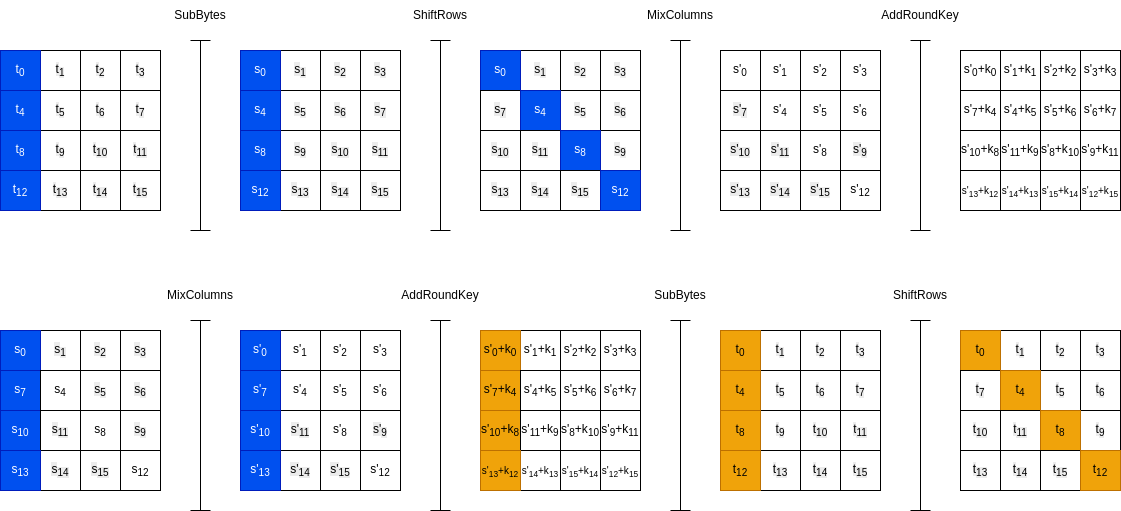
\includegraphics[width=0.75\textwidth]{img/sca/aes-distrace/attack_sbsr.png}

\end{frame}

\begin{frame}{Rappel sur le KeySchedule}
    \centering
    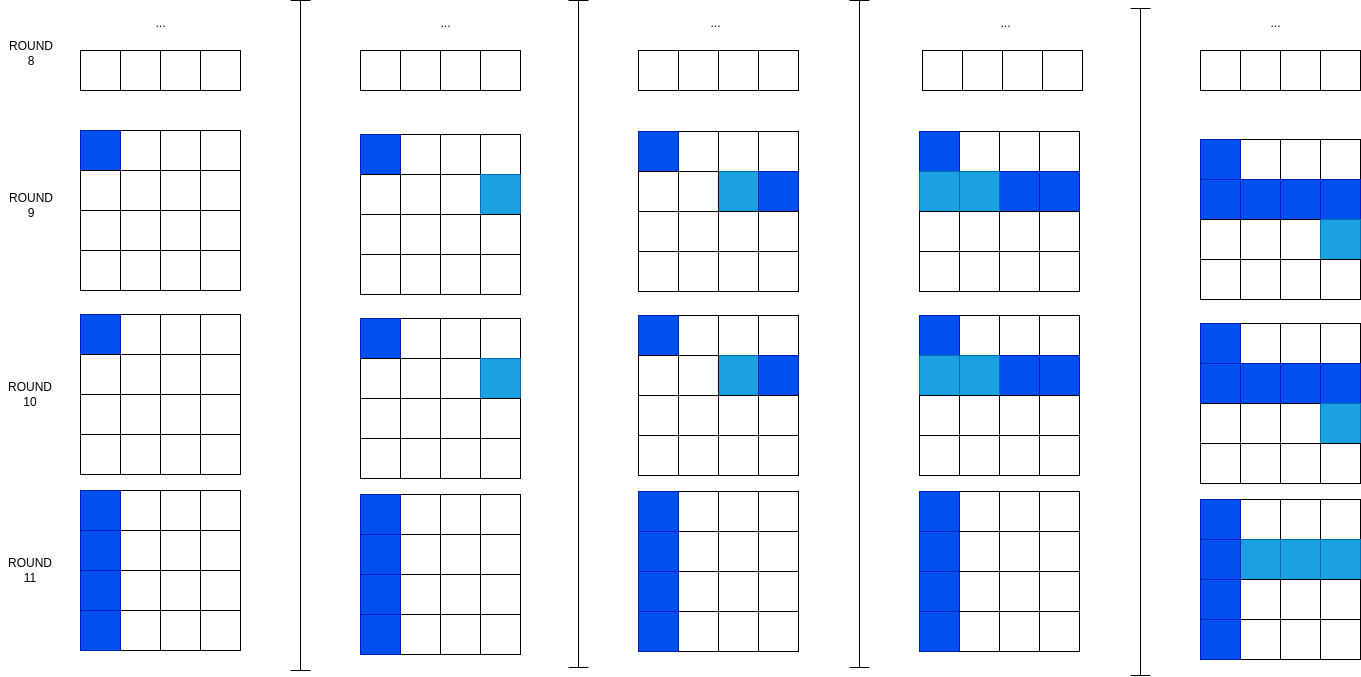
\includegraphics[width=0.23\textwidth,clip,trim=0 0 1070 0]{img/sca/aes-distrace/full_recovery.png}
    \pause
    \hspace{0.5cm}
    \raisebox{0.4cm}{\rule{0.4pt}{7cm}}
    \hspace{0.4cm}
    \hspace{0.5cm}
    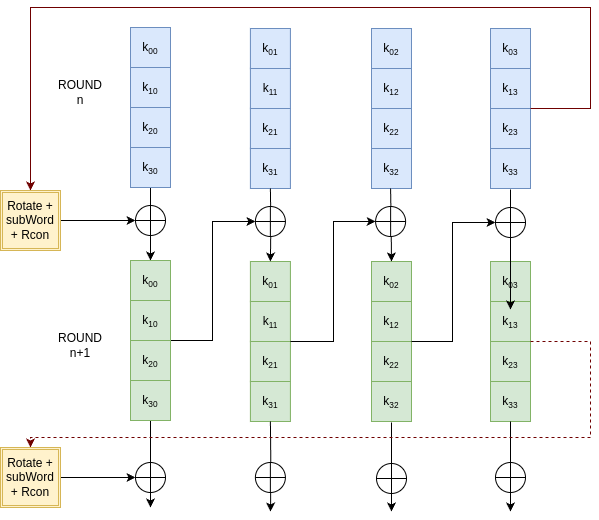
\includegraphics[width=0.6\textwidth]{img/sca/aes-distrace/keysched.png}
\end{frame}

\begin{frame}{Propagation de connaissance}
    \begin{columns}[T,onlytextwidth]
      \column{0.45\textwidth}
      \vspace{1cm}
        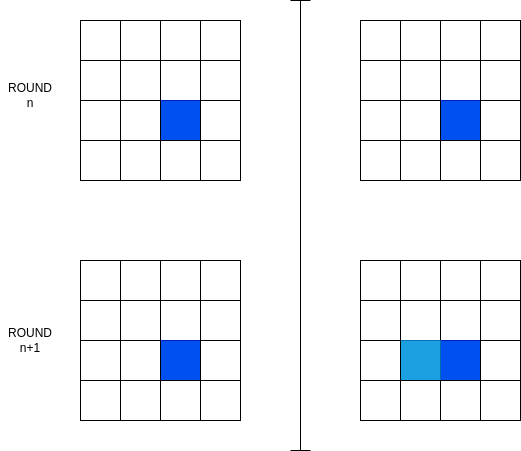
\includegraphics[width=\linewidth]{img/sca/aes-distrace/ex1.png}\\[1ex]
        \pause
      \column{0.45\textwidth}
        \vspace{1cm}
        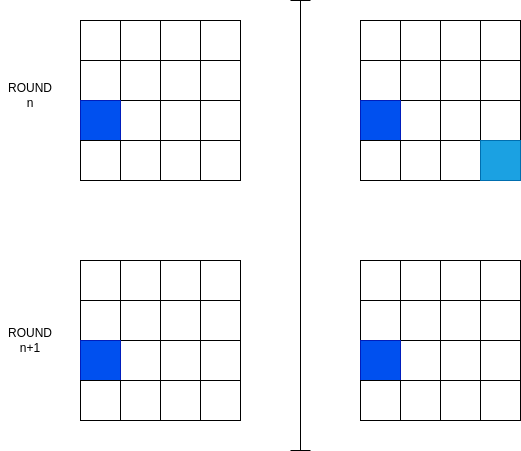
\includegraphics[width=\linewidth]{img/sca/aes-distrace/ex4.png}
    \end{columns}
\end{frame}


\begin{frame}{Full recovery}
    \begin{center}
        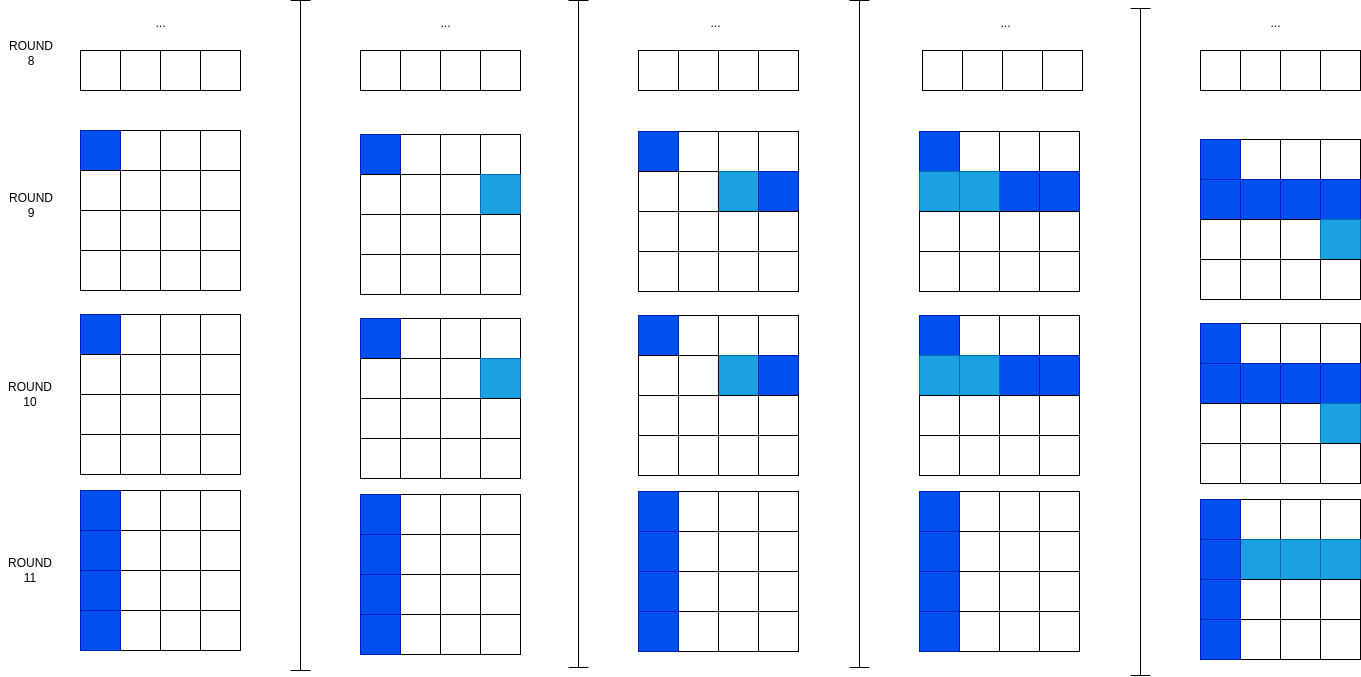
\includegraphics[width=0.85\textwidth]{img/sca/aes-distrace/full_recovery.png}
    \end{center}
    \pause
    
    Au final, il reste 3 bytes à bruteforcer (24 bits) \flag
\end{frame}
